\documentclass[conference]{IEEEtran}
\usepackage{graphicx}
\usepackage{booktabs}
\usepackage{array}
\usepackage{amsmath}

\begin{document}

\title{Interoperability, Portability, and Federation of Scalable Web Services:
Deep Technical Analysis of a Pulumi-Based Multi-Cloud Infrastructure}

\author{
\IEEEauthorblockN{Nikola Dinevski}
\IEEEauthorblockA{ndinevski5@gmail.com}
}

\maketitle

\begin{abstract}
This paper presents an extended engineering case study of interoperability and portability for scalable web services using Infrastructure as Code (IaC). The implementation uses Pulumi with TypeScript and targets two cloud platforms, Amazon Web Services (AWS) and Microsoft Azure, from a single codebase. The project deploys three compute styles (virtual machine, serverless, and Kubernetes) for the same renderer workload and evaluates portability at architecture, configuration, deployment, and operations levels. The analysis demonstrates that strong portability is achievable when service intent is separated from provider implementation through a shared contract, a unified configuration schema, and a provider factory pattern. At the same time, the paper shows that networking semantics, IAM/security models, and service-specific deployment primitives remain major adaptation points. A federation roadmap is proposed for active-active multi-cloud operation with unified traffic, identity, observability, and policy controls.
\end{abstract}

\begin{IEEEkeywords}
Interoperability, Portability, Federation, Infrastructure as Code, Pulumi, Multi-Cloud, AWS, Azure, EKS, AKS, Lambda, Function App, Kubernetes
\end{IEEEkeywords}

\section{Introduction}
Modern scalable web services are expected to be cloud-native, fault-tolerant, and operationally efficient. In practice, these systems are frequently built around one provider and later face strategic pressure to migrate, replicate, or federate across providers. The central challenge is balancing speed of delivery with long-term infrastructure independence.

In the context of the course \textit{Interoperability, Portability and Federation of Scalable Web Services}, this project investigates a realistic scenario: a Puppeteer-based PDF rendering platform implemented with one IaC codebase and deployed to both AWS and Azure.

Unlike papers that focus only on runtime performance, this work focuses on \textit{portability engineering}. The main question is not only ``which service is faster'', but ``how architecture choices determine migration effort and multi-cloud readiness''.

\section{Problem Statement and Motivation}
Organizations building scalable web services often encounter the following constraints:
\begin{itemize}
    \item dependence on provider-specific constructs (lock-in),
    \item costly migration due to non-portable deployment logic,
    \item duplicated operational tooling for each cloud,
    \item inconsistent security and compliance controls.
\end{itemize}

The motivation of this work is to design an IaC architecture where the business capability (document rendering as a web service) remains stable while the infrastructure implementation can change between providers with controlled effort.

\section{Research Goals and Questions}
The primary goal is to evaluate whether the current Pulumi architecture provides practical cross-cloud portability and a foundation for federation.

The study addresses the following questions:
\begin{itemize}
    \item \textbf{RQ1}: Which infrastructure elements are directly portable between AWS and Azure?
    \item \textbf{RQ2}: Which elements require provider-specific implementation and why?
    \item \textbf{RQ3}: What is the effective migration path from AWS to Azure (and vice versa)?
    \item \textbf{RQ4}: Which design changes are needed to move from provider switching to real federation?
\end{itemize}

\section{Methodology}
The paper uses a design-science and case-study methodology:
\begin{enumerate}
    \item analyze the implemented Pulumi codebase and abstractions,
    \item map functional components across AWS and Azure,
    \item identify portability-preserving and portability-breaking decisions,
    \item define migration and federation procedures,
    \item synthesize practical recommendations.
\end{enumerate}

The evaluation is qualitative-technical (architecture and process depth) with concrete implementation evidence from the project structure.

\section{Project and Workload Context}
The workload is a Puppeteer renderer exposed as web endpoints. The same logical service is deployed with three compute paradigms:
\begin{itemize}
    \item \textbf{VM model}: containerized renderer on a Linux VM,
    \item \textbf{Serverless model}: renderer function package,
    \item \textbf{Kubernetes model}: renderer container as a deployment + service.
\end{itemize}

This tri-model design is relevant for portability analysis because each paradigm has different abstraction leakage:
\begin{itemize}
    \item VMs are closer to OS-level portability,
    \item serverless is highly provider-shaped,
    \item Kubernetes provides a relatively portable workload layer but non-portable cluster provisioning.
\end{itemize}

\section{IaC Architecture in Detail}
\subsection{Core Architectural Pattern}
The infrastructure implementation uses an explicit abstraction strategy:
\begin{itemize}
    \item \textbf{Contract layer}: interface \texttt{CloudProvider} with \texttt{deploy()} as a stable provisioning entry point.
    \item \textbf{Selection layer}: \texttt{CloudProviderFactory} selects provider implementation from one key (\texttt{cloud}).
    \item \textbf{Configuration layer}: \texttt{InfrastructureConfig} centralizes shared settings.
    \item \textbf{Provider layer}: \texttt{AwsCloudProvider} and \texttt{AzureCloudProvider} contain cloud-specific logic.
    \item \textbf{Output layer}: shared output model exports uniform integration values (URLs, names, kubeconfig, notes).
\end{itemize}

This is a strong separation-of-concerns design where intent and implementation are decoupled.

\subsection{Configuration Model and Merge Strategy}
The configuration system merges defaults with stack overrides. This is critical because portability depends on how many values stay unchanged across migrations.

Portable shared keys include:
\begin{itemize}
    \item renderer image, container port, environment map,
    \item VM sizing intent,
    \item serverless runtime/handler/memory/timeout,
    \item Kubernetes scaling parameters,
    \item common tags and project naming.
\end{itemize}

The merge strategy supports deep overrides, enabling provider changes without rewriting the full stack configuration.

\subsection{Output Contract for Operational Interoperability}
A major practical feature is output normalization. Independent of cloud, deployment returns:
\begin{itemize}
    \item VM public IP and container URL,
    \item function service name and URL,
    \item cluster name and kubeconfig,
    \item Kubernetes service name.
\end{itemize}

This allows CI scripts, smoke tests, and user tooling to operate with minimal provider awareness.

% Optional Figure 1:
% Add a diagram: "Code architecture view" with five layers
% (Contract, Factory, Config, Provider Implementations, Outputs).

\section{Detailed Component-Level Analysis}
\subsection{Networking Layer}
Networking is conceptually portable but structurally different:
\begin{itemize}
    \item AWS uses VPC, subnets, route table associations, internet gateway, security groups.
    \item Azure uses virtual network, subnets, network interface, public IP, network security group.
\end{itemize}

Both achieve the same end state (publicly reachable services and isolated private addressing), but cloud resource composition differs. Therefore, networking is semantically portable, not syntactically portable.

\subsection{VM Component (EC2 vs Azure VM)}
\subsubsection{Implementation Details}
Both providers deploy a Linux virtual machine and bootstrap Docker automatically:
\begin{itemize}
    \item AWS uses EC2 with \texttt{userData} shell bootstrap.
    \item Azure uses Linux VM with base64-encoded \texttt{customData} script.
\end{itemize}

The renderer container is pulled and launched with environment variables and port mapping.

\subsubsection{Portability Characteristics}
Portability is medium-high. The container workload is identical, but script details differ:
\begin{itemize}
    \item package manager and Docker installation commands,
    \item default OS image choices,
    \item VM size naming conventions,
    \item NIC/public IP attachment model.
\end{itemize}

\subsection{Serverless Component (Lambda vs Function App)}
\subsubsection{Implementation Details}
The serverless path exposes the strongest provider divergence:
\begin{itemize}
    \item AWS deploys \texttt{lambda.Function} with a function URL and IAM role attachment.
    \item Azure deploys a Function App requiring storage account, service plan, package blob, and app settings.
\end{itemize}

Both run Node.js runtime and consume shared environment variables, but deployment pipelines are materially different.

\subsubsection{Portability Characteristics}
Portability is medium-low at IaC primitive level, medium-high at business capability level:
\begin{itemize}
    \item same intent: stateless request-driven rendering endpoint,
    \item different resource chains and packaging semantics,
    \item different auth and identity defaults.
\end{itemize}

\subsection{Kubernetes Component (EKS vs AKS)}
\subsubsection{Implementation Details}
Both providers provision managed Kubernetes clusters and then deploy the same renderer workload model:
\begin{itemize}
    \item deployment with container image and env vars,
    \item service exposing renderer over stable port mapping,
    \item configurable replicas and node sizing.
\end{itemize}

\subsubsection{Portability Characteristics}
Kubernetes offers a split portability profile:
\begin{itemize}
    \item \textbf{high portability} for Kubernetes manifests,
    \item \textbf{low-medium portability} for cluster provisioning, identity, networking integration, and node-pool semantics.
\end{itemize}

\subsection{Identity and Access Management}
Identity is the least portable component:
\begin{itemize}
    \item AWS IAM roles/policies are explicit and service-granular.
    \item Azure relies on managed identities, role assignments, and service-specific access policies.
\end{itemize}

The architecture correctly isolates this in provider implementations, but this layer still demands provider expertise during migration.

\section{Portability Layer Model}
For a deeper analysis, portability can be decomposed into five layers:
\begin{enumerate}
    \item \textbf{Source portability}: one TypeScript codebase for all providers.
    \item \textbf{Configuration portability}: shared stack schema with limited cloud-specific keys.
    \item \textbf{Artifact portability}: same container image and mostly shared runtime artifacts.
    \item \textbf{Runtime portability}: equivalent public interfaces despite different internals.
    \item \textbf{Operational portability}: normalized outputs and tests for both providers.
\end{enumerate}

If each layer is assigned a relative portability score, a simple aggregate model can be expressed as:
\[
P = \sum_{i=1}^{5} w_i \cdot p_i, \quad \sum_{i=1}^{5} w_i = 1
\]
where $p_i$ is the portability quality of layer $i$ and $w_i$ is its importance for the organization.

\section{AWS--Azure Capability Mapping}
\begin{table}[h]
\centering
\resizebox{\columnwidth}{!}{%
\begin{tabular}{|p{2.1cm}|p{2.2cm}|p{2.3cm}|p{2.8cm}|p{1.4cm}|}
\hline
{}\textbf{Domain} & \textbf{AWS Resource(s)} & \textbf{Azure Resource(s)} & \textbf{Portability Comment} & \textbf{Score} \\
\hline
Network core & VPC, subnets, IGW, routes & VNet, subnets, NSG, NIC & Same concept, different composition & High \\
VM host & EC2 + SG + userData & VM + NSG + customData & Script/OS adaptation required & Medium \\
Serverless core & Lambda + IAM + URL & Function App + Plan + Storage & Highest structural divergence & Medium-Low \\
K8s workload & Deployment/Service via provider & Deployment/Service via provider & Workload spec highly portable & High \\
K8s control plane & EKS + node group & AKS + agent pool & Provisioning semantics differ & Medium \\
Identity & IAM roles/policies & Managed identity + RBAC & Least portable area & Low \\
Outputs/API & Pulumi outputs & Pulumi outputs & Strong common integration surface & High \\
\hline
\end{tabular}%
}
\caption{Detailed AWS--Azure Mapping and Relative Portability}
\label{tab:detailed_mapping}
\end{table}

\section{Migration Playbook (Provider Switching)}
Migration in this architecture is designed as controlled switching rather than full rewrite.

\subsection{Step-by-Step Procedure}
\begin{enumerate}
    \item Select stack and set \texttt{cloud} target.
    \item Configure provider region/location.
    \item Provide provider-specific credentials and secrets.
    \item Validate artifact paths (container image, function package).
    \item Run \texttt{pulumi preview} to inspect plan.
    \item Run \texttt{pulumi up} for deployment.
    \item Execute smoke tests using normalized outputs.
\end{enumerate}

\subsection{Deployment Evidence}
\begin{figure}[h]
\centering
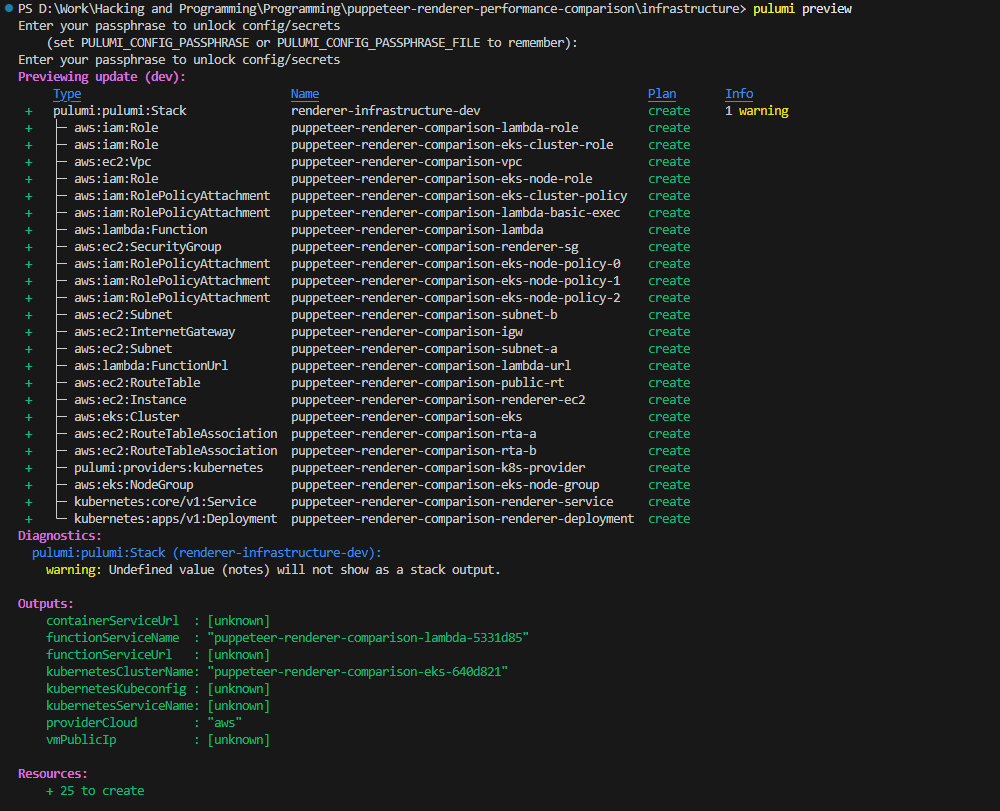
\includegraphics[width=\columnwidth]{pulumi-preview-aws.png}
\caption{Pulumi preview plan for AWS stack.}
\label{fig:pulumi_preview_aws}
\end{figure}

\begin{figure}[h]
\centering
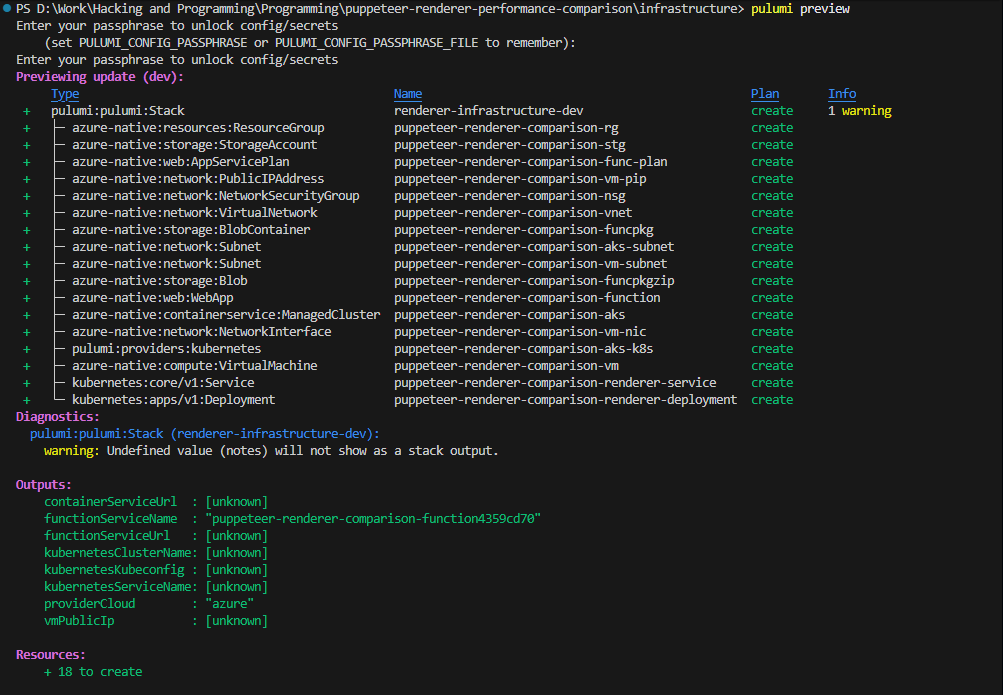
\includegraphics[width=\columnwidth]{pulumi-preview-azure.png}
\caption{Pulumi preview plan for Azure stack.}
\label{fig:pulumi_preview_azure}
\end{figure}

\subsection{Minimal Configuration Delta}
\begin{table}[h]
\centering
\begin{tabular}{|p{3.2cm}|p{4.3cm}|}
\hline
{}\textbf{Change Category} & \textbf{Update Required} \\
\hline
Cloud target & \texttt{renderer-infrastructure:cloud} \\
Location & \texttt{aws:region} or \texttt{azure-native:location} \\
Secrets & provider auth and secure values (e.g. VM admin password) \\
Service intent & typically unchanged (image/port/env/replicas) \\
Post-deploy validation & endpoint checks and basic rendering test \\
\hline
\end{tabular}
\caption{Provider Migration Delta in Practice}
\label{tab:migration_delta}
\end{table}

\section{Testability and CI/CD Implications}
The project includes provider-focused tests that verify resource creation and output behavior with Pulumi mocks. This is important for portability because regressions often happen in provider glue code, not in business logic.

A robust multi-cloud CI workflow should include:
\begin{itemize}
    \item unit tests for config merging,
    \item provider contract tests for both AWS and Azure,
    \item preview drift checks per stack,
    \item endpoint smoke tests after deployment.
\end{itemize}

\section{Security and Compliance View}
From a portability perspective, security must be standardized at policy level while allowing provider-specific enforcement mechanisms.

Recommended approach:
\begin{itemize}
    \item define baseline controls independent of cloud (least privilege, encrypted secrets, restricted ingress),
    \item implement controls with native primitives in each provider,
    \item validate controls through policy-as-code and deployment checks.
\end{itemize}

This avoids weakest-link migration where security posture degrades during provider switching.

\section{Cost and Operational Trade-Offs}
Even with equivalent topology, cost behavior differs by provider due to pricing models, billing units, and managed service overhead. Therefore, portability must include economic validation, not only technical deployment success.

Operationally, the architecture reduces repeated engineering work through shared definitions. However, platform expertise is still needed for tuning IAM, networking, and serverless limits.

\section{Federation Roadmap (Beyond Switching)}
The current implementation uses one active provider per stack. True federation requires simultaneous operation across providers.

\subsection{Target Federated Model}
\begin{itemize}
    \item active-active endpoints in AWS and Azure,
    \item global traffic management with health-aware failover,
    \item unified identity federation for operators and automation,
    \item centralized observability across clouds,
    \item harmonized policy and compliance controls.
\end{itemize}

\subsection{Phased Evolution Plan}
\begin{enumerate}
    \item \textbf{Phase 1}: keep switching model, harden tests and outputs.
    \item \textbf{Phase 2}: deploy both providers in parallel environments.
    \item \textbf{Phase 3}: introduce global routing and failover.
    \item \textbf{Phase 4}: add unified telemetry, SLOs, and policy gatekeeping.
\end{enumerate}

% Optional Figure 2:
% Add "Federation reference architecture":
% Users -> Global DNS/Traffic Manager -> AWS endpoints + Azure endpoints,
% with shared observability and policy plane.

\section{Limitations}
This case study is strong in architectural depth but has the following limitations:
\begin{itemize}
    \item focus on two providers only (AWS/Azure),
    \item qualitative portability evaluation without long-term production telemetry,
    \item serverless packaging path may evolve with platform updates,
    \item no full active-active traffic benchmark included in current stage.
\end{itemize}

\section{Conclusion}
This extended analysis confirms that the Pulumi-based architecture provides substantial practical portability for scalable web services across AWS and Azure. The key success factor is architectural discipline: a stable provider contract, unified configuration model, and cloud-isolated implementation modules.

The most portable assets are service intent, workload artifacts, and output contracts. The least portable assets are IAM, cloud-native service plumbing, and control-plane provisioning. Therefore, migration is not ``free'', but it is transformed from an ad-hoc rewrite into an engineered and testable workflow.

For the subject of interoperability, portability, and federation, this project demonstrates a realistic and academically relevant direction: use IaC abstraction to minimize lock-in, then progressively evolve from provider switching to true cross-cloud federation.

\begin{thebibliography}{99}

\bibitem{pulumi_docs}
Pulumi, ``Pulumi Documentation,'' 2026. [Online]. Available: https://www.pulumi.com/docs/

\bibitem{pulumi_patterns}
Pulumi, ``Component Resources and Abstraction Patterns,'' 2026. [Online]. Available: https://www.pulumi.com/docs/iac/concepts/components/

\bibitem{aws_well_arch}
Amazon Web Services, ``AWS Well-Architected Framework,'' 2024.

\bibitem{azure_well_arch}
Microsoft Azure, ``Microsoft Azure Well-Architected Framework,'' 2024.

\bibitem{k8s_docs}
The Kubernetes Authors, ``Kubernetes Documentation,'' 2026. [Online]. Available: https://kubernetes.io/docs/

\bibitem{eks_docs}
Amazon Web Services, ``Amazon EKS Documentation,'' 2026.

\bibitem{aks_docs}
Microsoft Azure, ``Azure Kubernetes Service (AKS) Documentation,'' 2026.

\bibitem{lambda_docs}
Amazon Web Services, ``AWS Lambda Developer Guide,'' 2026.

\bibitem{azure_func_docs}
Microsoft Azure, ``Azure Functions Documentation,'' 2026.

\bibitem{armbrust}
M. Armbrust et al., ``A View of Cloud Computing,'' \textit{Communications of the ACM}, vol. 53, no. 4, pp. 50--58, 2010.

\bibitem{cloud_portability}
E. Di Nitto, C. A. Ardagna, D. Petcu, and P. Mohagheghi, ``Cloud Portability and Interoperability,'' in \textit{Cloud Computing}, Springer, 2013.

\end{thebibliography}

\end{document}
